\section{Introduction}\label{s:intro}

% \TODO{
% This section includes the context and motivation behind the work, explicitly or implicitly highlights the main research question(s), provides a high-level explanation of the solution, and describes the contributions.}

% \TODO{Context, motivation, research question asds, and original contribution could be organized in subsections.}


Rewriting software components; or entire systems; in a different language is a common practice to address various limitations caused by the original implementation language, including but not limited to performance, maintainability, and scalability. The primary motivation behind rewriting is to leverage the strengths of the new language to address the limitations of the original language. However, rewriting a large system, especially in a different language with potentially different paradigms can be a complex and time-consuming task. This study aims to asses the viability of leveraging language interoperability to simplify and expedite the rewriting process.

Most well known major software services today like Facebook, YouTube, Google, LinkedIn, Wordpress, etc. have all had either components many of them starting out with language such as PHP or Ruby on Rails because these were the popular choices back in the day and what the intial developers where likely the most familiar with. We can take YouTube as a good example, it was intially written largely in PHP, but as the platform grew this came with some key drawbacks, a key one being scalability, one reason for switching to Python (and C++) was because Python speifically had both a wider range of syntax expressions and more importantly a better optimizability. This allowed for rapid flexible development and deployment, in addition to scalability and performance at an improved maintainability over PHP.\  

Similar stories exist for so many other platforms, as languages evolve and the second system effect comes into play we will naturally see software evolve to adapt to new requirements and technologies as developers realize their mistakes of the past. Though the rewriting process does not come without its own set of challenges. It could be argued that a contributing factor to the downfall of the Netscape browser was the decision to do a ground up rewrite of the browser, a reason for this being that the original code base was so messy developers did not want to contribute \textcite{pogue2000netscape}. The choice was then made to start from new, but by the time the browser released it still lacked a lot of basic features \textcite{zawinski1999resignation}. 

More broadly speaking the manner in which we choose to rewrite software in a different language should preferably align with the core motivation as best as we can, while mitigating as many of the downsides as possible. This is where the concept of language interoperability could come into play. Language interoperability can potentially offer some very interesting benefits, a key one being the ability to effectively implement a gradual/iterative rewrite while still allowing for the original code to be used. The benefit here being that we can leverage the strengths of the new language, still use existing familiar infrastructure, all while allowing the system to be iteratively improved without there being any major downtime untill the rewrite is complete.

\begin{lstlisting}
    //Example of interoperability between C and C++
    #include <iostream>
    extern "C" {
        #include <stdio.h>
        void c_function() {
            printf("Hello from C\n");
        }
    }
    int main() {
        c_function();
        std::cout << "Hello from C++" << std::endl;
        return 0;
    }
\end{lstlisting}

% ---------- templates for figures ----------------------- 

% \begin{figure}[bh]
%     %% The macro `\onecolgrid' is defined in `vusec.sty'
%     %% NOTE: The suffix "./figures/" is implicitly included for this relative path.
%     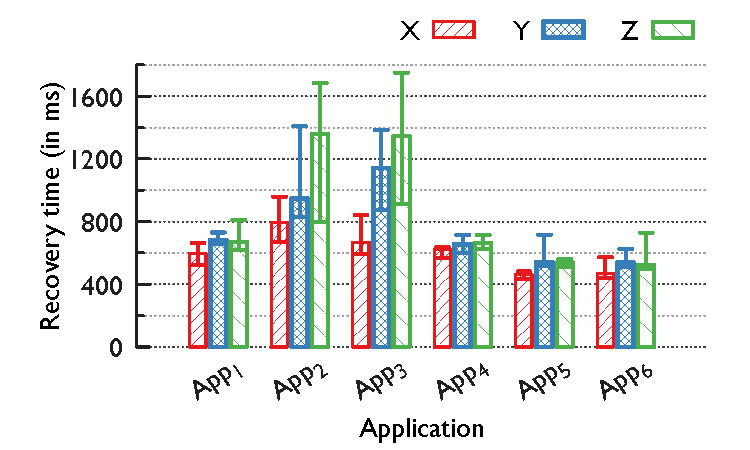
\includegraphics[width=\onecolgrid]{cache-by-app}
%     %% Labels should immediately follow caption, to keep latex quiet.
%     \figcap{Simple one-column figure. Please include a brief explanation or takeaway.}\label{fig:1col}
% \end{figure}

% \begin{figure*}[th]
%     %% The macro `\threecolgrid' is defined in `vusec.sty'
%     \begin{subfigure}[t]{\threecolgrid}
%         %% NOTE: The suffix "./figures/" is implicitly included for these relative paths.
%         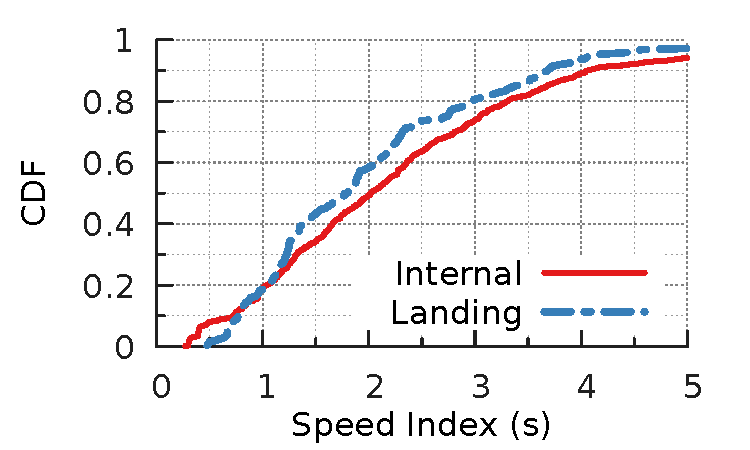
\includegraphics[width=\linewidth]{three-col/speed_index}
%         \sfigcap{}\label{fig:3col-a}
%     \end{subfigure}
%     \begin{subfigure}[t]{\threecolgrid}
%         %% NOTE: You do not have to mention the extension.
%         %% (The example figures are in PDF format.)
%         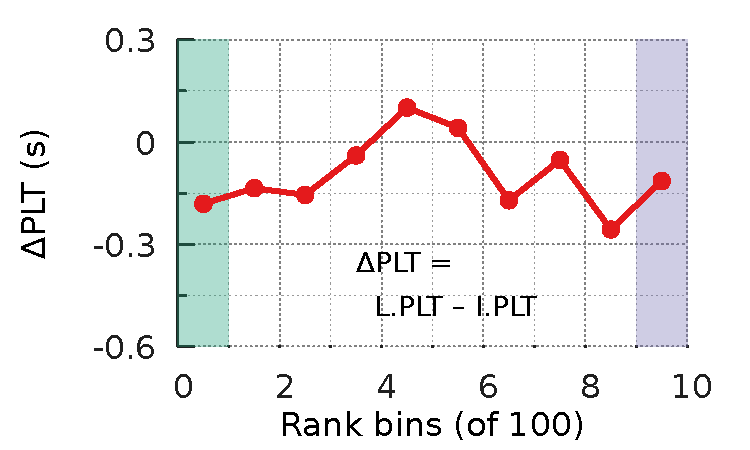
\includegraphics[width=\linewidth]{three-col/plt_ranks_diff}
%         \sfigcap{}\label{fig:3col-b}
%     \end{subfigure}
%     \begin{subfigure}[t]{\threecolgrid}
%         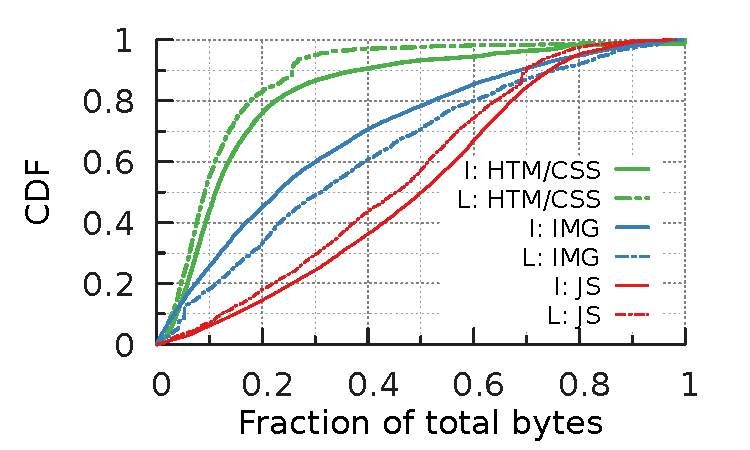
\includegraphics[width=\linewidth]{three-col/mimes}
%         \sfigcap{}\label{fig:3col-c}
%     \end{subfigure}
%     %% Labels should immediately follow caption, to keep latex quiet.
%     \figcap{Generate clear and beautiful figures (in PDF) that can be rendered side by side while still being easy to read and interpret. Choose colors wisely from the colorbrewer2.org website.}\label{fig:3col}
% \end{figure*}

% \begin{table}[hb]
%     \centering
%     \tabcap{A simple table describing the characteristics of a data set or the results of an experiment}\label{tab:sample}
%     \taburulecolor{black!45}
%     \begin{tabu}{c|c|r|r|r|r}
%         \toprule
%         \multirow{2}{*}{\thead{Char.}} &
%             \multirow{2}{*}{\thead{\#samples}} &
%             \thead{Count} &
%             \multicolumn{3}{c}{\thead{Perf. Score}}\\
%         &
%             &
%             \thead{of items} &
%             \thead{X} & \thead{Y} & \thead{Z} \\
%         \midrule
%         \stress{P}
%             & 214 & 56 & 9 & 23 & 24 \\
%         \stress{Q}
%             & 117 & 27 & 7 & 10 & 10 \\
%         \stress{R}
%             & 222 & 11 & 6 & 4 & 1 \\
%         \stress{S}
%             & 187 &  9 & 1 & 6 & 2 \\
%         \stress{T}
%             & 180 & 16 & 7 & 5 & 4 \\
%         \bottomrule
%     \end{tabu}

% \end{table}

 